\chapter{LTE}\label{lte}
Mobile communications is on to its \ac{4G} of network infrastructure with \ac{LTE}. This network infrastructure is an improvement upon \ac{UMTS}, which is a \ac{3G} network. \ac{LTE} has \ac{DL} speeds of up to 300 Mbit/s and \ac{UL} speeds of 75 Mbit/s. This development was driven by the users want of faster download speeds for mobile services such as Video Streaming.

\section{Self-Organising Network}\label{self organising network}
\ac{SON}~\cite{feng2008self}

\section{Handover}\label{handover}
The process of handover is very important in mobile telecommunications. It involves moving the resource allocation for a mobile phone or a piece of \ac{UE} from one base station to another. This process is used to provide more \ac{QoS} to customers by allowing them to continue to use provided services even after moving out of range of the original serving base station. To keep with the QoS it is important that handovers are done fast, have little-to-no disruption to the users experience and are completed with a very high success rate. If a handover is unsuccessful it is likely that an on going call will be dropped due to there not being enough resources available on a base station, known as an \ac{eNodeB} in \ac{LTE}, or the received signal strength to the \ac{UE} drops below a certain threshold needed to maintain the call. Handovers are stated to take roughly 0.25 seconds to complete after the decision has been made for a handover to take place~\cite{3gpp2012triggers}.

\subsection{Parameters}\label{parameters}
In LTE there are two main parameters that are used in the handover process. These parameters are the \ac{TTT} and \ac{hys}. The hys is used to define how much better the \ac{RSS} of a neighbouring base station must be than the serving base station for a handover to be considered. The values of hys are defined in \ac{dB} and range from 0 to 10 dB in 0.5 dB increments, this results in there being 20 different values of hys. The full range of hys values can be seen in Table~\ref{tab:hys}.

\begin{table}[H]
  \begin{center}
    \begin{tabular}{| l | p{2cm} |}
  	  \hline
      Parameter & Value(dB) \\ \hline
      hys & 0.0 \newline
	  0.5 \newline
	  1.0 \newline
	  1.5 \newline
	  2.0 \newline
	  2.5 \newline
	  3.0 \newline
	  3.5 \newline
	  4.0 \newline
	  4.5 \newline
	  5.0 \newline
	  5.5 \newline
	  6.0 \newline
	  6.5 \newline
	  7.0 \newline
	  7.5 \newline
	  8.0 \newline
	  8.5 \newline
	  9.0 \newline
	  9.5 \newline	  	  	  	  
	  10.0 \\
      \hline
  	\end{tabular}
  \end{center}
  \caption{Table of the different LTE hys values.}
  \label{tab:hys}
\end{table}

\begin{table}[H]
  \begin{center}
    \begin{tabular}{| l | p{1.5cm} |}
  	  \hline
      Parameter & Value(s) \\ \hline
      TTT & 0.0 \newline
      0.04 \newline
	  0.064 \newline
	  0.08 \newline
	  0.1 \newline
	  0.128 \newline
	  0.16 \newline
	  0.256 \newline
	  0.32 \newline
	  0.48 \newline
	  0.512 \newline
	  0.64 \newline
	  1.024 \newline
	  1.280 \newline
	  2.56 \newline
	  5.12 \\
      \hline
  	\end{tabular}
  \end{center}
  \caption{Table of the different LTE TTT values.}
  \label{tab:ttt}
\end{table}

\begin{figure}[H]
  \begin{center}
    	  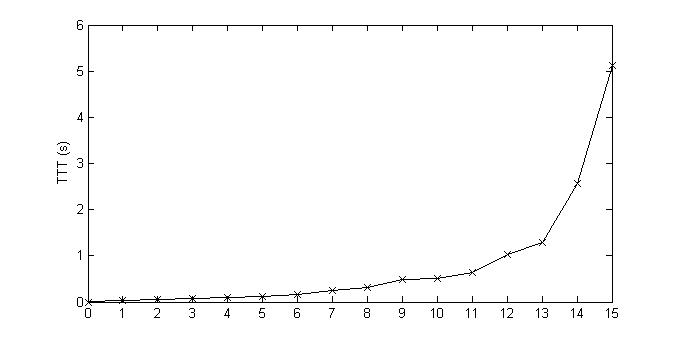
\includegraphics[width=0.5\textwidth]{figures/TTTgraph.jpg}
    \end{center}
    \caption{Graph of TTT values.}
    \label{fig:ttt}
\end{figure}
\subsection{Procedure}\label{procedure}
\begin{table}[H]
  \begin{center}
    \begin{tabular}{| l | p{11.1cm} |}
  	  \hline
      Event Type & Trigger Criteria \\ \hline
      A1 & Serving becomes better than a threshold. \\
      A2 & Serving becomes worse than a threshold. \\
      A3 & Neighbour becomes offset better than PCell. \\
      A4 & Neighbour becomes better than threshold. \\
      A5 & PCell becomes worse than threshold1 and neighbour becomes better than threshold2. \\
      A6 & Neighbour becomes offset better than SCell. \\
      B1 & Inter RAT neighbour becomes better than threshold. \\
      B2 & PCell becomes worse than threshold1 and inter RAT neighbour becomes better than threshold2. \\
      \hline
  	\end{tabular}
  \end{center}
  \caption{Table of the different LTE Trigger types and their criteria.}
  \label{tab:trigger}
\end{table}
\ac{PCell} \ac{SCell}

~\cite{3gpp2012triggers}
~\cite{cox2012introduction}